%!TEX TS-program=xelatex
\documentclass[xetex]{beamer}

\usefonttheme{professionalfonts}
\usepackage[UTF8]{ctex}
\usepackage{hyperref}
\usepackage{unicode-math}
\usepackage{amsmath, amssymb}
\usepackage{graphicx, wrapfig}
\usepackage{nopageno}

\DeclareMathOperator{\argmax}{argmax}

\usetheme[block=fill, subsectionpage=progressbar]{metropolis}

\setmathfont{XITS Math}

%这是标题页
\title{重积分}
\subtitle{曲面面积}
\author{数学分析MOOC小组}
%这是标题页

\begin{document}

\frame{\maketitle}

%这是第一页
\begin{frame}
    \frametitle{一般方程表示法}
    曲面方程为
    $$z=f(x,y), \quad (x,y) \in D$$
    曲面面积表达式为
    $$S = \iint \limits_D \sqrt{1 + f _x ^2 (x,y) + f _y ^2 (x,y)} dxdy$$
\end{frame}

\begin{frame}
    \frametitle{例题}
    \begin{figure}[ht]
        \centering %图片居中放置
        % 在这里使用 \includegraphics 插入图片,改变width就可以改变图片的大小。
       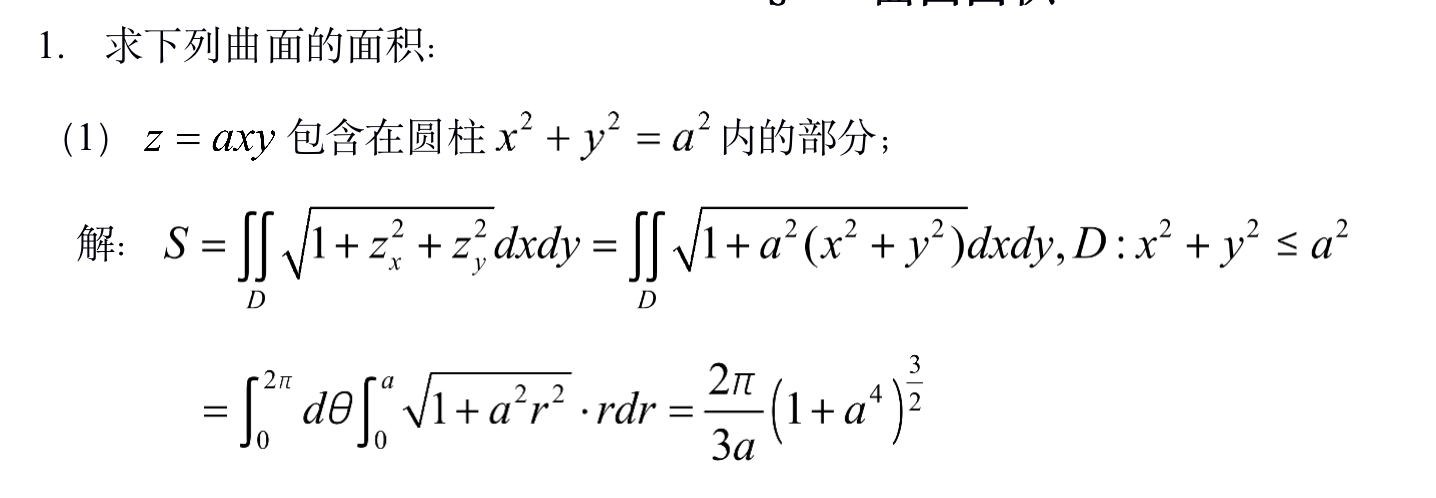
\includegraphics[width=1.0\textwidth]{img/a.jpg}
    \end{figure}
\end{frame}

\begin{frame}
    \frametitle{参数方程表示法}
    曲线方程为
    $$x = x(u,v), \quad y=y(u,v), \quad z=z(u,v), \quad (u,v) \in D $$
    曲面面积为
    $$S = \iint \limits_D \sqrt{EG-F^2} dudv$$
    其中
    $$r_u = \left( \dfrac{\partial x} {\partial u} , \dfrac{\partial y} {\partial u} ,\dfrac{\partial z} {\partial u} \right)$$
    $$r_v = \left( \dfrac{\partial x} {\partial v} , \dfrac{\partial y} {\partial v} ,\dfrac{\partial z} {\partial v} \right)$$
\end{frame}

\begin{frame}
    \frametitle{参数方程表示法}
    $$E = | r_u | ^2 = \left( \frac{\partial x} {\partial u} \right) ^2 + \left( \frac{\partial y} {\partial u} \right) ^2 + \left( \frac{\partial z} {\partial u} \right) ^2 $$ \\
    $$G = | r_u | ^2 = \left( \frac{\partial x} {\partial v} \right) ^2 + \left( \frac{\partial y} {\partial v} \right) ^2 + \left( \frac{\partial z} {\partial v} \right) ^2 $$ \\
    $$F = \left( r_u \cdot r_v \right) = \frac{\partial x} {\partial u} \frac{\partial x} {\partial v} + \frac{\partial y} {\partial u} \frac{\partial y} {\partial v} +\frac{\partial z} {\partial u} \frac{\partial z} {\partial v} $$
\end{frame}

\begin{frame}
    \frametitle{例题}
    \begin{figure}[ht]
        \centering %图片居中放置
        % 在这里使用 \includegraphics 插入图片,改变width就可以改变图片的大小。
       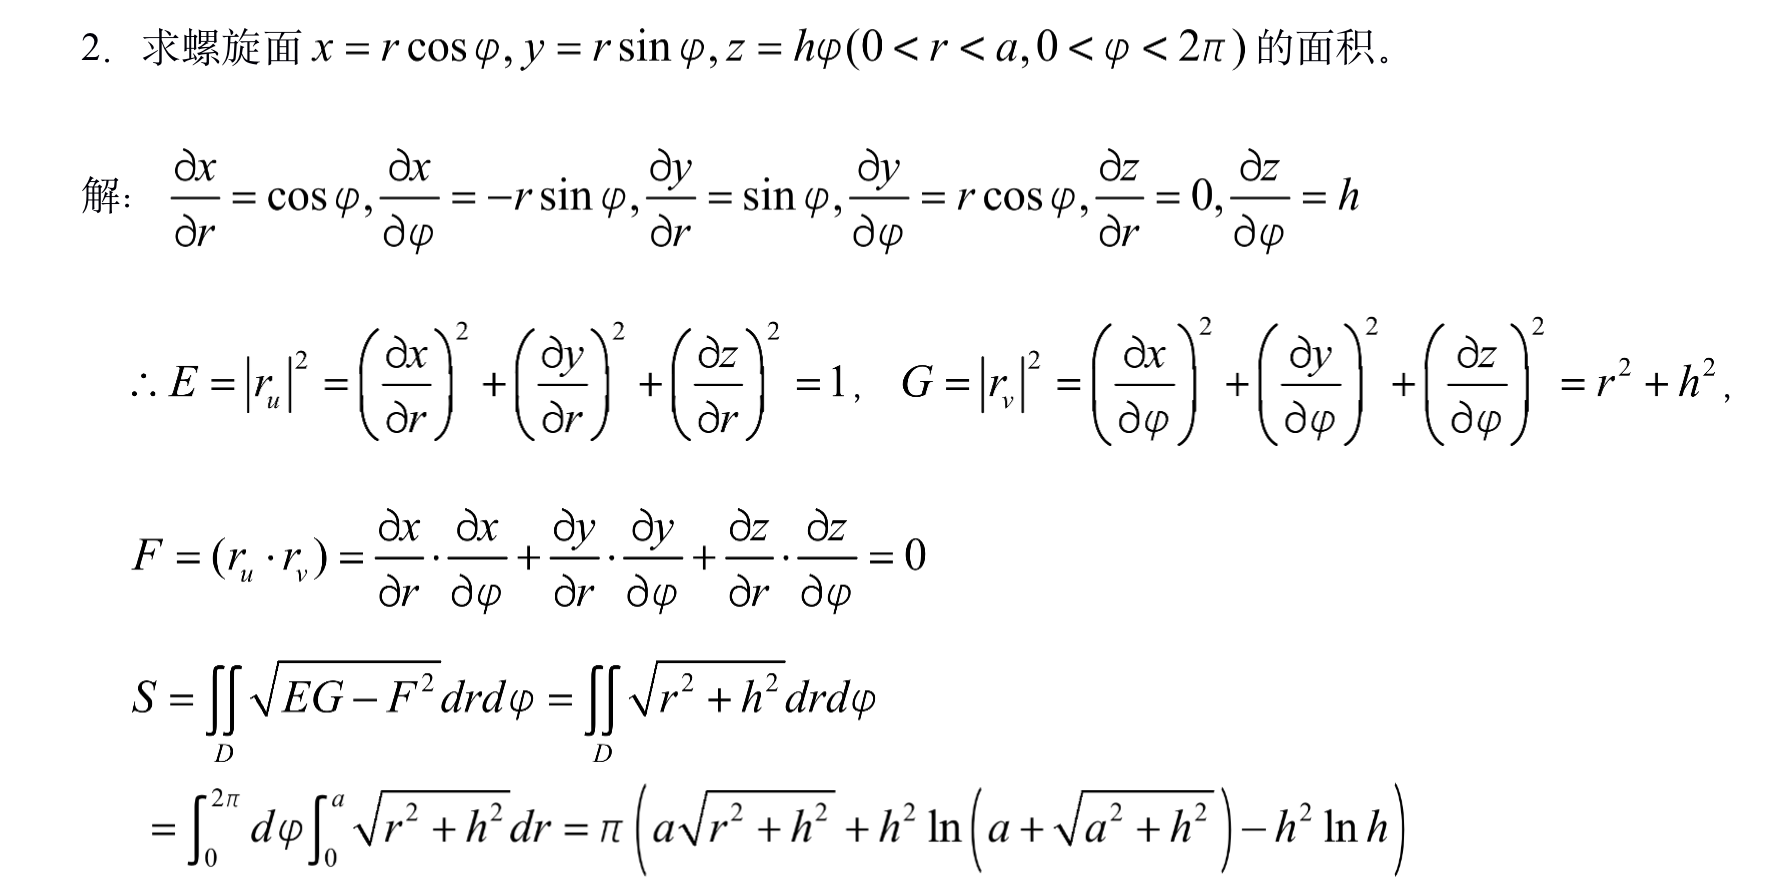
\includegraphics[width=1.2\textwidth]{img/b.jpg}
    \end{figure}
\end{frame}

\begin{frame}
    \frametitle{例题}
    \begin{figure}[ht]
        \centering %图片居中放置
        % 在这里使用 \includegraphics 插入图片,改变width就可以改变图片的大小。
       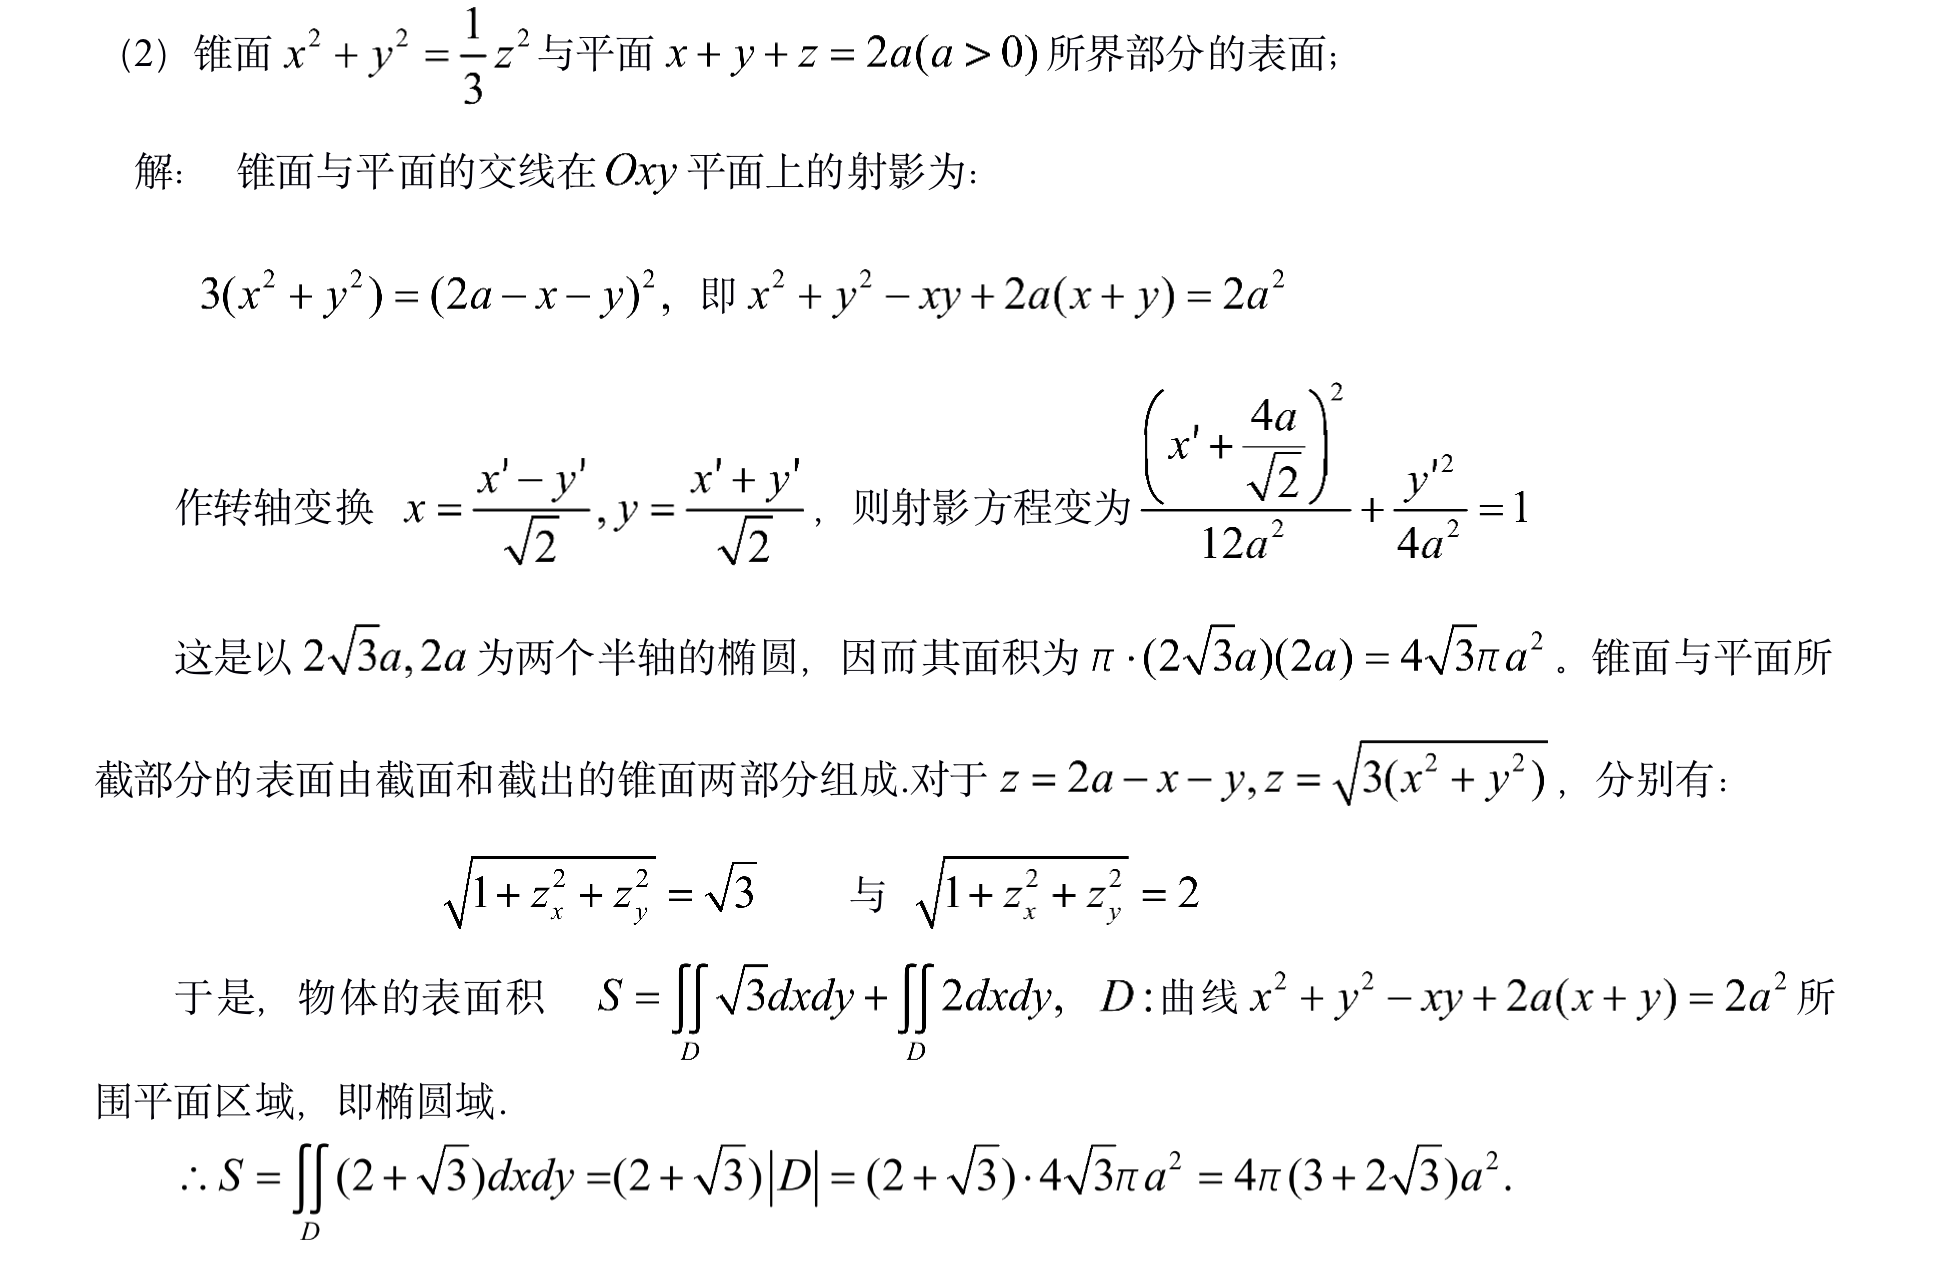
\includegraphics[width=1.1\textwidth]{img/c.jpg}
    \end{figure}
\end{frame}

\begin{frame}
    \frametitle{例题}
    \begin{figure}[ht]
        \centering %图片居中放置
        % 在这里使用 \includegraphics 插入图片,改变width就可以改变图片的大小。
       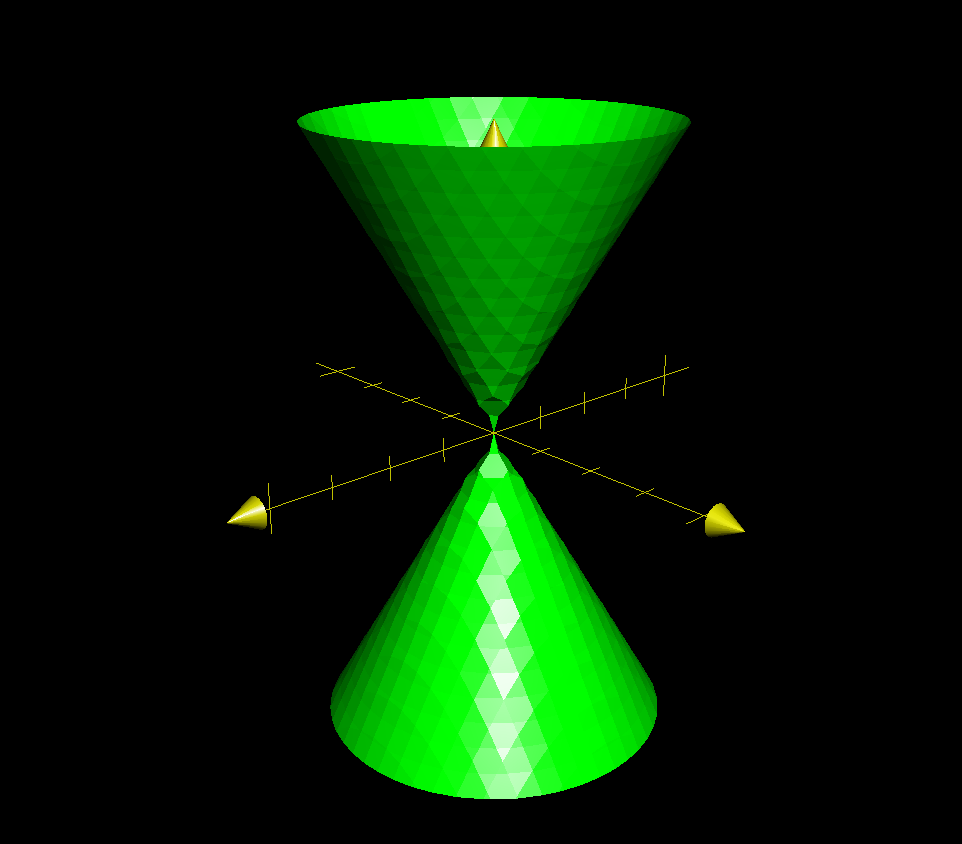
\includegraphics[width=0.8\textwidth]{img/d.jpg}
    \end{figure}
\end{frame}

\begin{frame}
    \section{谢谢观看!}
\end{frame}

\end{document}
